% ==========================================================================
% CM3070 Computer Science Final Project — Preliminary Report
% Iliass Jabali — Student Number 230586639
% Template: CM3020 Project Idea 1 — Governing Multiple Models Around a Goal
% Project: Hyrox Personal Coach
% ==========================================================================

\documentclass[11pt,a4paper]{report}

\usepackage[utf8]{inputenc}
\usepackage[T1]{fontenc}
\usepackage{lmodern}
\usepackage{microtype}
\usepackage[margin=2.5cm]{geometry}
\usepackage{setspace}
\onehalfspacing
\usepackage{parskip}
\usepackage{graphicx}
\usepackage{booktabs}
\usepackage{array}
\usepackage{tabularx}
\usepackage{caption}
\usepackage{float}
\usepackage{tikz}
\usetikzlibrary{arrows.meta, positioning, fit, backgrounds, calc}
\usepackage{listings}
\usepackage{xcolor}
\definecolor{codegray}{rgb}{0.96,0.96,0.96}
\definecolor{codeblue}{rgb}{0.1,0.3,0.6}
\definecolor{codegreen}{rgb}{0.0,0.5,0.0}
\lstdefinelanguage{TypeScript}{
  keywords={const, let, var, function, return, if, else, for, while, async, await,
           import, export, from, default, type, interface, class, extends, implements,
           public, private, protected, static, readonly, new, this, true, false, null, undefined,
           enum, throw, try, catch, finally, of, in},
  keywordstyle=\color{codeblue}\bfseries,
  ndkeywords={string, number, boolean, any, void, Promise, Array, z},
  ndkeywordstyle=\color{codegreen}\bfseries,
  sensitive=true,
  comment=[l]{//},
  morecomment=[s]{/*}{*/},
  commentstyle=\color{gray}\ttfamily,
  stringstyle=\color{red!60!black}\ttfamily,
  morestring=[b]',
  morestring=[b]"
}
\lstset{
  basicstyle=\ttfamily\footnotesize,
  backgroundcolor=\color{codegray},
  frame=single,
  breaklines=true,
  showstringspaces=false,
  tabsize=2,
  captionpos=b,
  xleftmargin=4pt,
  xrightmargin=4pt
}

\usepackage[colorlinks=true, linkcolor=black, citecolor=blue, urlcolor=blue]{hyperref}
\usepackage{cite}

\title{
  \vspace{-2cm}
  \Large\textbf{CM3070 Computer Science Final Project} \\[0.2cm]
  \Large\textbf{Preliminary Report} \\[1cm]
  \LARGE\textbf{Hyrox Personal Coach} \\[0.3cm]
  \large Multi-Model LLM Orchestration for Hybrid-Sport Training \\[2cm]
}
\author{
  Iliass Jabali \\
  Student Number: 230586639 \\[0.4cm]
  BSc Computer Science \\
  University of London \\[0.4cm]
  Template: CM3020 Project Idea 1 \\
  \emph{Governing Multiple Models Around a Goal}
}
\date{\today}

\begin{document}

\maketitle

\thispagestyle{empty}
\chapter*{Word Counts}
\addcontentsline{toc}{chapter}{Word Counts}

\begin{table}[H]
\centering
\begin{tabular}{lrr}
\toprule
\textbf{Chapter} & \textbf{Words} & \textbf{Limit} \\
\midrule
1. Introduction              & $\sim$\,930   & 1000 \\
2. Review of Existing Solutions    & $\sim$\,1660  & 2500 \\
3. System Design             & $\sim$\,1510  & 2000 \\
4. Prototype Implementation  & $\sim$\,1410  & 1500 \\
\midrule
\textbf{Total}           & \textbf{$\sim$\,5510} & \textbf{6000} \\
\bottomrule
\end{tabular}
\end{table}

\textit{Counts measured with \texttt{texcount -inc}, excluding the title page, section headers, captions, tables, code listings, figures, references, and the AI-use declaration. Each chapter is within its per-chapter limit and the total is within the strict 6000-word overall limit.}

\tableofcontents

% ==========================================================================
% Chapter 1: Introduction (target ~950 words, max 1000)
% ==========================================================================

\chapter{Scope and Context}
\label{ch:introduction}

\section{Concept and contribution}

This project designs a personal AI training companion for athletes competing in Hyrox, a hybrid-fitness race format that combines running with functional strength workouts. The system ingests an athlete's recent training history from their existing Strava and Garmin accounts, computes structured features such as heart-rate zones, training load, and acute-to-chronic workload ratio, and produces a next-session recommendation as schema-validated JSON. The reasoning is performed by three distinct pre-trained large language models, each used in a different prompted agent role: a small model classifies sessions, a large model generates coaching guidance, and a mid-size model critiques that guidance for plausibility and safety. A custom orchestrator, written in TypeScript and built directly on the Vercel AI SDK, handles routing, retries, and conflict resolution between agents. The technical contribution is not any single model but the deliberate orchestration discipline applied to a domain that has historically been served either by static plans or by single-model chat coaches.

\section{Template and requirements}

This project follows \textbf{CM3020 Project Idea 1: Multi-Model Orchestration for a Target Outcome}, operating across different domains or data spaces, into a single workflow that solves a well-specified problem. It explicitly does not require model training; the contribution is in model selection, integration, software engineering, and rigorous evaluation. The template flags that simply running models is not enough: markers expect evidence of testing, rejection, and substitution as part of the development process.

The present project meets these requirements as follows. Three pre-trained models are used: Anthropic's Claude Haiku, Claude Sonnet, and Claude Opus, each in a distinct prompted role. The three roles --- classification, generation, and critique --- operate over structurally different reasoning tasks even though the underlying data domain is shared. The integration is a custom TypeScript orchestrator built on the Vercel AI SDK, deliberately avoiding higher-level agent frameworks so that the orchestration logic itself constitutes the technical contribution. Schema validation between agents is enforced by Zod at runtime. Evaluation prioritises objective metrics --- classifier accuracy, output consistency, and ablation studies --- with a small user study as a supplementary signal, following direct guidance from the project supervisor.

\section{Motivation and need}

Hyrox is a hybrid-fitness race comprising 8\,km of running interspersed with 8 functional workout stations such as sled pushes, burpee broad jumps, and wall balls. It is currently among the fastest-growing fitness sports globally, with reported participation more than doubling year on year since 2022 \cite{hyrox_growth}. The athlete population is expanding rapidly while access to expert coaching has not kept pace.

Athletes currently choose between two unsatisfactory options. The first is following a generic static training plan distributed as a PDF or spreadsheet; such plans ignore the athlete's individual data entirely and treat training as open-loop control over an inherently stochastic biological system. The second is paying a human coach, typically between EUR\,150 and EUR\,300 per month, which is inaccessible to most amateur athletes. Meanwhile, the athlete's own wearables already record everything a coach would need to reason about: heart-rate variability, sleep, resting heart rate, acute and chronic load, pace distributions, and perceived exertion. The data exists; the missing layer is intelligent, individualised reasoning over it.

Recent advances in large language models suggest that this reasoning layer is now technically feasible at low cost. However, naively wrapping a single chat model around a system prompt has documented failure modes: hallucinated training volumes, inconsistent recommendations between sessions, and an inability to handle the multi-modal nature of hybrid sport, in which running load and strength load interact in non-additive ways. A more rigorous approach is required, and that is what this project proposes.

\section{Goal and objectives}

This project sets out to determine whether a multi-agent orchestration of distinct pre-trained large language models, grounded in structured biometric features and constrained by schema validation, can produce coaching guidance that is consistent, plausible, and useful to Hyrox athletes.

To meet this aim, the project pursues four objectives:

\begin{enumerate}
  \item Design and implement a data ingestion and feature engineering layer that converts raw Strava and Garmin exports into structured features relevant to hybrid-sport training load.
  \item Design and implement a three-agent orchestration pipeline with distinct large language models in distinct prompted roles, schema-validated outputs, and explicit conflict resolution between agents.
  \item Evaluate the system using objective metrics --- classifier accuracy, output consistency, prompt-variant and Critic ablations --- as the primary signal, supplemented by a small user study with consenting adult athletes.
  \item Critically compare the resulting system to both the multi-agent LLM orchestration literature and existing AI-based fitness applications, articulating how the architecture differs and what gap it addresses.
\end{enumerate}

\section{Scope and boundaries}

The system is deliberately scoped. It targets a single sport (Hyrox), a single athlete population (consenting healthy adults), and read-only ingestion of pre-existing wearable data. It produces training guidance and never medical or clinical claims; a permanent disclaimer is presented in the user interface. The user study is small in scale (five to ten participants) and supplementary; the primary evaluation is offline and objective. These constraints reflect both feasibility for a single student over the project duration and direct supervisory guidance.

\section{Structure of this report}

The rest of this preliminary report proceeds as follows. Chapter~\ref{ch:lit-review} surveys two strands of prior work: multi-agent LLM orchestration systems from recent research, and existing AI-based fitness coaching applications. Each is critiqued and the two are then synthesised to identify the gap this project addresses. Chapter~\ref{ch:prototype} turns to the feature prototype. Chapter~\ref{ch:design} comes first, laying out the system design: it defines the evaluation strategy and work plan, specifies the schemas, maps each agent to its role, and details the orchestration architecture. Together they answer what this project takes on.

% ==========================================================================
% Chapter 2: Literature Review (target ~2460 words, max 2500)
% Structure: research question, branch A, branch B, synthesis & bridge
% ==========================================================================

\chapter{Background research and related initiatives}
\label{ch:lit-review}

\section{Research question and scope of review}

This review is organised around a single research question that anchors what to read, what to critique, and where to bridge to the project:

\begin{quote}
\textit{How do existing multi-agent large-language-model orchestration systems and AI-based fitness coaching applications address structured reasoning over personal training data, and what architectural and evaluation gaps remain for hybrid-sport athletes?}
\end{quote}

Two branches of literature are directly relevant. The first is the recent body of work on multi-agent orchestration of large language models, in which systems compose multiple model calls under explicit control logic to overcome the limitations of single-call prompting. The second is the longer-established field of AI-based fitness applications, which has matured from static recommender systems toward adaptive coaching products and, more recently, toward LLM-driven chat coaches. Both branches are treated critically below, and a final synthesis identifies the architectural and evaluation gap this project occupies.

\section{Branch A: Multi-agent LLM orchestration}

\subsection{Reasoning frameworks and actionable outputs in LLMs}

ReAct, proposed by Yao et al.~\cite{yao2022react}, showed that weaving chain-of-thought steps together with tool calls yields large improvements over either technique alone on knowledge-intensive tasks. The contribution is foundational: it established that a language model can productively be treated as a reasoning controller that issues tool calls, rather than as a black-box answer generator. ReAct's evaluation, however, is concentrated on factual question-answering benchmarks such as HotpotQA and FEVER, and on agent benchmarks such as ALFWorld and WebShop. The original work uses a single model for both reasoning and acting, and offers no guidance on when to delegate distinct reasoning roles to distinct models. It also makes no provision for schema-validated structured outputs, which are central to any system operating in a domain where downstream consumers (other agents, user interfaces, safety checks) require reliable contracts. These two omissions --- role specialisation and structured output validation --- are directly addressed by the present project.

\subsection{Self-criticism and reflection as an agent primitive}

Reflexion, introduced by Shinn et al.~\cite{shinn2023reflexion}, extends the agent paradigm by adding a self-critique loop: the agent reflects on failed attempts, stores verbal feedback in episodic memory, and conditions future attempts on that feedback. Reflexion materially improves performance on coding and decision-making benchmarks, and is conceptually close to the Critic role used in the present project's pipeline. The critical weakness, acknowledged by the authors, is that self-reflection depends on a usable signal of failure. In coding tasks this is provided by unit-test output; in open-ended domains such as training-plan generation, no analogous environmental signal exists by default. The present project responds to this gap by encoding plausibility and safety rules into the Critic agent's prompt, transforming reflection from an introspective exercise into a rule-grounded check. This is a small but deliberate architectural choice: it treats the Critic not as a self-reflecting model but as a separate role-specialised judge.

\subsection{Multi-agent debate and structured disagreement}

Du et al.~\cite{du2023debate} show that having multiple LLM instances debate and revise their answers improves factuality and reasoning quality on reasoning benchmarks. The mechanism is essentially structured disagreement: each agent sees the others' arguments and updates its own. The result challenges the common assumption that additional compute should always be spent on deeper single-agent reasoning rather than across multiple agents. A genuine architectural weakness of the work, however, is that the agents are identical model copies debating in symmetric roles. The question of whether \emph{distinct} models in \emph{distinct} roles can outperform symmetric debate at fixed compute is left open. The present project's use of three different Claude models (Haiku, Sonnet, Opus) in three non-symmetric roles (classify, generate, critique) is, in part, a small probe of that gap. The choice is also motivated by cost: paying Opus prices for a session-classification task that Haiku can do reliably is a waste of budget that no production-grade orchestrator should accept.

\subsection{Framework-level orchestration}

At the systems level, AutoGen~\cite{wu2023autogen} offers a general toolkit for composing conversational agents that can invoke tools and message one another. LangGraph and similar industry frameworks have since adopted a directed-graph view of agent control flow. These frameworks are powerful, and they have undoubtedly accelerated the adoption of multi-agent patterns in industry, but their published evaluations focus on demonstrating the framework rather than on rigorous ablations of architectural choices. There is also a recurring mismatch between the abstractions these frameworks supply and the small, controllable, schema-validated orchestrators required for high-stakes domains such as health-adjacent coaching. The present project deliberately uses a hand-rolled TypeScript orchestrator with Zod schemas rather than adopting a framework, both to retain explicit control over routing, retries, and validation, and to preserve the orchestration logic itself as the technical contribution. Framework adoption would shift the contribution from \emph{architecture} to \emph{configuration}, which would not meet the template's requirement for technical depth.

\subsection{Common weaknesses across the orchestration literature}

Three weaknesses recur across the orchestration literature reviewed above. First, evaluation is dominated by benchmark accuracy, with little attention to \emph{consistency}: whether the same input produces the same output across repeated runs. In a coaching context where user trust is built on stability of advice from one session to the next, consistency arguably matters more than raw accuracy. Second, almost all systems use a single model across all roles, leaving role-specialisation by model size, latency profile, or cost tier under-explored. Third, structured output validation --- forcing model outputs through a schema before they are passed to the next agent --- is rare in the academic literature, despite being standard in production agent systems. These three gaps directly shape the present project's commitments and are revisited in the synthesis below.

\section{Branch B: AI-based fitness coaching}

\subsection{Platform-led training plans}

Strava is the dominant social fitness platform. Its own training-plan offering has changed materially since the preliminary report was written: in April 2025 Strava announced its acquisition of Runna, a personalised running-training app, and now surfaces Runna-generated plans rather than a purely static, goal-and-date-parameterised template~\cite{strava_runna}. This is a genuine strength --- Runna's plans adapt to logged performance and schedule --- but the adaptation is confined to a single modality, running, which is precisely the limitation this review returns to across every product surveyed below. The strength of the Strava approach remains reach and data availability: more athletes use Strava than any single device manufacturer's app. Its weakness, even post-acquisition, is that closed-loop adaptation is offered for running only; a Hyrox athlete's strength and sled sessions receive no comparable treatment. The sports-science literature has long shown that closed-loop adaptive approaches outperform open-loop ones on equivalent populations~\cite{busso2003}, and the present project closes that loop for the specific, currently unaddressed case of hybrid-sport training: the Coach agent receives the athlete's actual recent data, across all logged modalities, on every planning cycle.

\subsection{Adaptive coaching from wearables}

Garmin Coach, supported by Firstbeat analytics, represents the state of the art in commercial adaptive coaching~\cite{firstbeat_whitepaper}. It ingests heart-rate variability and training-status signals derived from years of physiological research and adapts daily workouts accordingly. The right physiological signal is being used, and the underlying load model is well grounded. The critical limitation is sport scope: Garmin Coach is locked to running, cycling, and swimming. Hybrid sport, in which strength work and running interact in non-additive ways, is not supported. The underlying load model is TRIMP-based, which is well established for endurance training but is documented to underweight strength-dominant sessions~\cite{strength_load_critique}. For a Hyrox athlete whose race performance depends on both endurance and strength, a load model that ignores half the training is a structural problem, not a calibration one.

\subsection{AI-driven coaching startups}

A more recent cohort of startups --- including Humango and Athletica --- explicitly markets AI-driven adaptive coaching. Humango remains single-modality, endurance-focused. Athletica has since extended its supported-sport list to include Hyrox alongside running, triathlon, cycling, and rowing~\cite{humango,athletica}, which means the sport-coverage gap identified in the preliminary report no longer holds against this specific competitor and the critique must be sharpened rather than repeated unchanged. Published technical material for both remains sparse, but where available the architecture is a single conversational AI coach analysing wearable data and suggesting adjustments, not a disclosed multi-model pipeline with an explicit, separately-reasoning critique stage; Athletica's own documentation states the coach ``does not automatically modify your training'' without human confirmation, which is a design choice for user control but also evidence that verification, where it exists, is manual rather than architectural. Both products are closed-source subscriptions, which is a legitimate commercial choice but limits academic critique to what public documentation permits. The gap the present project addresses is therefore not merely ``no product covers Hyrox'' --- Athletica now does --- but that no covering product is open, auditable, or built on role-specialised models with a schema-validated, independently-reasoning critique step; that architectural and evaluation gap, not sport coverage alone, is what the rest of this review substantiates.

\subsection{Generic LLM coaching applications}

A large number of consumer apps now wrap a single general-purpose chat model in a fitness-themed system prompt. The advantage is rapid development; the documented disadvantage is severe hallucination~\cite{huang2023hallucination}. Fabricated training volumes, confused race formats, and physiologically implausible recommendations are well documented in user reports and in the broader LLM-hallucination literature. The absence of structured inputs and outputs makes these systems essentially impossible to evaluate or constrain rigorously. They form the lower bound against which any serious LLM-coaching system, including this project, must be compared --- not because they represent the state of the art but because they represent what naive LLM adoption looks like and what serious work must visibly exceed.

\subsection{The hybrid-sport gap}

Across the fitness branch, three gaps stand out specifically for Hyrox, revised here from the preliminary report to reflect that Hyrox is no longer entirely without commercial coverage: Athletica now lists it as a supported sport. First, coverage does not equal a well-grounded load model: the major running-derived and TSS-derived systems still under-represent strength and sled work even where a Hyrox mode has been added, because the underlying training-load mathematics was not designed for it. Second, none of the commercial products, including Athletica, are open or auditable --- their coaching logic, whatever its internal structure, is not published, which makes them poor scientific baselines and difficult to critique on methodological rather than product grounds. Third, none combines transparent, well-grounded load modelling with the structured-reasoning and explicit-critique advantages of recent LLM orchestration work; where a critique or safety check exists, as in Athletica, it is a manual user-confirmation step rather than a second model reasoning independently over the plan. The present project's gap is therefore architectural and evaluative, not a claim that no product has ever mentioned Hyrox.

\section{Synthesis and bridge to the project}

The two branches of literature reviewed above are usually treated separately, but it is their synthesis that motivates this project. The orchestration literature shows that combining distinct LLM calls under explicit control yields gains in factuality, reasoning, and reliability over single-call prompting, but its evaluation rarely targets domains with strong domain priors and few benchmark labels. The fitness coaching literature, conversely, has strong domain priors and rich biometric data, but its leading commercial systems are either rigid (Strava), single-modality (Garmin), or opaque (Humango, Athletica), and the generic LLM-wrapper apps fail because they discard structure altogether.

This project sits in the unaddressed intersection. It applies the architectural lessons of the orchestration literature --- distinct models in distinct roles, schema-validated outputs, explicit critique --- to the structured biometric data that the fitness literature has long understood how to compute. The novelty is not any single model, nor any single feature, but the deliberate combination of orchestration discipline with sports-science feature engineering, applied to a sport (Hyrox) that no commercial system currently serves well.

Three concrete commitments follow from this synthesis and shape the rest of the report. First, the system uses three deliberately different Claude models in three deliberately different roles, as a small probe of the role-specialisation gap identified in the orchestration literature and as a cost-tiered architectural choice. Second, every agent output is validated against a Zod schema before being passed downstream, addressing the structured-output gap. Third, the evaluation emphasises consistency and ablation alongside accuracy, addressing the consistency gap identified in the orchestration literature and acting on direct supervisory guidance to prioritise objective metrics over user-reported satisfaction.

% ==========================================================================
% Chapter 3: Design (target ~1950 words, max 2000)
% ==========================================================================

\chapter{System Design}
\label{ch:design}

\section{Domain analysis and user model}

The system targets a specific user: a healthy adult Hyrox athlete who already records workouts to Strava and wears a Garmin device. The user wants concrete next-session guidance grounded in their actual data, not generic recommendations. They are technically literate enough to authorise an OAuth connection but should not need to interpret raw biometric data themselves. Their reading habits during a training week are short: a one-screen weekly plan with a clear rationale is the target deliverable, not a research dashboard.

Three design properties are optimised for. The first is \emph{transparency} --- the user can always see why a recommendation was made, both at the session-classification level and at the planning level. The second is \emph{safety} --- recommendations are checked before being shown, never produced silently. The third is \emph{consistency} --- the same data should yield similar advice on repeated runs, because user trust depends on stability of advice over time rather than on its peak quality on any single run. These three properties drive the architectural decisions described in the rest of this chapter.

\section{System Blueprint}

The architecture is a directed pipeline with five components, deployed as a single Next.js application written in TypeScript:

\begin{enumerate}
  \item \textbf{Ingestion layer.} Pulls workout sessions from Strava and Garmin via OAuth (currently CSV import in the prototype) and persists raw activity records.
  \item \textbf{Feature engineering layer.} Pure TypeScript. Converts raw sessions into structured features including pace zones, heart-rate zones, TRIMP (training impulse), and acute-to-chronic workload ratio (ACWR).
  \item \textbf{Agent pipeline.} Three prompted Claude agents (Classifier, Coach, Critic) called in sequence, each producing Zod-validated JSON consumed by the next stage.
  \item \textbf{Orchestrator.} Custom TypeScript code that routes data between agents, retries on schema failure, and resolves conflicts when the Critic rejects or revises the Coach's output.
  \item \textbf{Presentation layer.} A minimal Next.js page that renders the resulting weekly plan, the per-session classification, and the Critic's rationale.
\end{enumerate}

Figure~\ref{fig:architecture} illustrates the data flow. The orchestrator (not shown explicitly) sits beneath the agent pipeline and is the project's principal technical contribution.

\begin{figure}[H]
\centering
\resizebox{\textwidth}{!}{%
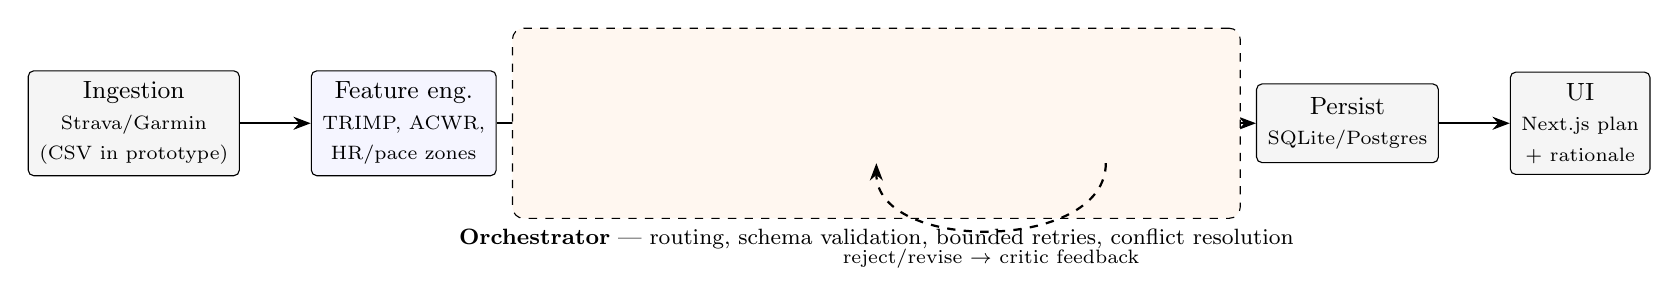
\begin{tikzpicture}[
  font=\small,
  node distance=6mm and 9mm,
  box/.style={draw, rounded corners=2pt, align=center, minimum height=10mm, inner sep=4pt, fill=blue!4},
  agent/.style={box, fill=green!7, minimum width=20mm},
  io/.style={box, fill=gray!8},
  flow/.style={-{Stealth[length=2.2mm]}, thick},
]
  % Main left-to-right pipeline
  \node[io] (ingest) {Ingestion\\\scriptsize Strava/Garmin\\\scriptsize (CSV in prototype)};
  \node[box, right=of ingest] (feat) {Feature eng.\\\scriptsize TRIMP, ACWR,\\\scriptsize HR/pace zones};
  \node[agent, right=of feat] (clf) {Classifier\\\textbf{Haiku}};
  \node[agent, right=of clf] (coach) {Coach\\\textbf{Opus}};
  \node[agent, right=of coach] (critic) {Critic\\\textbf{Sonnet}};
  \node[io, right=of critic] (persist) {Persist\\\scriptsize SQLite/Postgres};
  \node[io, right=of persist] (ui) {UI\\\scriptsize Next.js plan\\\scriptsize + rationale};

  \draw[flow] (ingest) -- (feat);
  \draw[flow] (feat) -- (clf);
  \draw[flow] (clf) -- node[above, font=\scriptsize] {Zod} (coach);
  \draw[flow] (coach) -- node[above, font=\scriptsize] {Zod} (critic);
  \draw[flow] (critic) -- (persist);
  \draw[flow] (persist) -- (ui);

  % Orchestrator band beneath the three agents
  \node[draw, dashed, rounded corners, fill=orange!6, fit=(clf)(coach)(critic),
        inner sep=7mm, label=below:{\footnotesize\textbf{Orchestrator} --- routing, schema validation, bounded retries, conflict resolution}] (orch) {};

  % Critic -> Coach revision feedback loop
  \draw[flow, dashed] (critic.south) to[out=-90, in=-90] node[below, font=\scriptsize, yshift=-1mm] {reject/revise $\rightarrow$ critic feedback} (coach.south);
\end{tikzpicture}%
}
\caption{System architecture; the pipeline runs from ingestion on the left to rendering on the right, and each agent's output is validated against a Zod schema (labelled \emph{Zod}) before the next stage consumes it. The orchestrator spans the three Claude agents and owns reliability: routing, schema-validation retries, and the reject/revise feedback loop that returns Critic feedback to the Coach.}
\label{fig:architecture}
\end{figure}

\section{Agent role design and model selection}

A core architectural choice is the deliberate use of three different Claude models in three different roles. The choice follows the cost--capability spectrum: Claude Haiku is the fastest and least expensive, Claude Opus is the most capable, and Claude Sonnet sits between them. Each role is matched to the model whose capability profile fits the task, not to the strongest available model. This is a small probe of the role-specialisation question raised in the orchestration literature and a deliberate cost-tiered design.

\subsection{Classifier (Claude Haiku)}

The Classifier receives a single session's structured features and assigns it to one of a small set of Hyrox-relevant labels: \texttt{run}, \texttt{strength}, \texttt{sled}, \texttt{burpees}, \texttt{hybrid}, \texttt{recovery}, or \texttt{other}. The label space is small and the reasoning required is shallow. Classification runs once per session, potentially on dozens of sessions per athlete, so cost and latency dominate, which makes Haiku the right model. The Classifier's output is validated against the \texttt{ClassifierOutput} schema and stored alongside the session.

\subsection{Coach (Claude Opus)}

The Coach receives the full athlete history --- typically 30 days of classified sessions plus aggregated features --- and produces a structured next-session recommendation: session type, duration, intensity zone, rationale, and any warnings. This is the most demanding reasoning step, because the model must reason simultaneously over load, fatigue, the athlete's hybrid-sport profile, and the Hyrox race calendar. Opus is chosen for this role. The Coach is invoked at most once per planning cycle, so the cost premium is bounded.

\subsection{Critic (Claude Sonnet)}

The Critic receives the Coach's recommendation along with the athlete's recent history and returns a verdict --- \texttt{approve}, \texttt{revise}, or \texttt{reject} --- with structured reasons. The Critic enforces a small set of hard rules encoded in its prompt: no consecutive maximum-intensity days, no recommendation that ignores a documented ACWR spike, no medical or clinical claims. Sonnet is chosen because careful rule application is required but Opus-level open-ended reasoning is not.

\section{Schemas and structured outputs}

Every agent output is validated at runtime against a Zod schema. This is a deliberate architectural commitment: the schema is the contract between agents, and an output that fails validation triggers a retry or a hard failure rather than silent downstream degradation. Listing~\ref{lst:zod} shows the principal schemas.

\begin{lstlisting}[language=TypeScript, caption={Representative Zod schemas. Each agent's output is validated against its schema before being passed to the next stage.}, label={lst:zod}]
import { z } from 'zod';

export const ClassifierOutput = z.object({
  sessionId: z.string(),
  label: z.enum(['run', 'strength', 'sled', 'burpees',
                 'hybrid', 'recovery', 'other']),
  confidence: z.number().min(0).max(1),
  rationale: z.string().min(10).max(300),
});

export const CoachOutput = z.object({
  sessionType: ClassifierOutput.shape.label,
  durationMinutes: z.number().int().min(15).max(180),
  intensityZone: z.enum(['Z1', 'Z2', 'Z3', 'Z4', 'Z5']),
  rationale: z.string().min(20).max(500),
  warnings: z.array(z.string()).default([]),
});

export const CriticOutput = z.object({
  verdict: z.enum(['approve', 'revise', 'reject']),
  reasons: z.array(z.string()).min(1),
  revisedPlan: CoachOutput.optional(),
});
\end{lstlisting}

Schema validation is not a presentation concern; it is a control-flow primitive. If the Classifier returns a label outside the enum, the orchestrator does not pass that output to the Coach. Instead, it retries with a more explicit prompt suffix and ultimately fails loudly rather than silently degrading.

The schemas above state the original design. During implementation the label set was deliberately narrowed to four values (\texttt{run}, \texttt{sled}, \texttt{burpees}, \texttt{mixed}) and \texttt{intensityZone}/\texttt{durationMinutes} were replaced by a free-text \texttt{focus} field, so that a small illustrative evaluation set could discriminate meaningfully between labels and so the Coach and Critic could exchange qualitative nuance a fixed enum would discard. This trade-off, and its consequence for how much structure the schema can now enforce, is evaluated critically in Chapter~\ref{ch:evaluation}.

\section{Orchestrator design}

The orchestrator is the project's main technical contribution and a small TypeScript module with three responsibilities. First, \emph{routing}: it calls Classifier $\to$ Coach $\to$ Critic in sequence, threading each agent's typed output into the next. Second, \emph{retries}: on a schema validation failure, it retries with an explicit ``the previous output did not match the required schema; correct it'' suffix, up to a small bounded number of attempts (currently three). Third, \emph{conflict resolution}: if the Critic returns \texttt{reject}, the orchestrator does not surface the Coach's original output to the user; if the Critic returns \texttt{revise} with a \texttt{revisedPlan}, the orchestrator surfaces the revision and records both versions for later evaluation.

The orchestrator is built directly on the Vercel AI SDK's model-call primitives, not on a higher-level agent framework such as LangGraph or AutoGen. This is a deliberate scoping decision discussed in Chapter~\ref{ch:lit-review}: framework adoption would shift the contribution from architecture to configuration and obscure the technical depth the template requires.

\section{Data layer}

Athlete data is stored in a local SQLite database during development and is intended to move to a managed Postgres instance for the user study. The schema separates raw activity records (immutable), engineered features (recomputable), and agent outputs (versioned). Versioning agent outputs is necessary for ablation: it must be possible to compare, for example, Coach prompt variant v1 against v2 on identical inputs, which requires retaining both outputs.

\section{Work plan and feasibility}

The work plan covers 22 weeks and is organised into eight phases: setup, prototype harness, literature review and design, preliminary report and prototype video (week 7), full system build (weeks 7--14), user study and objective evaluation (weeks 14--17), draft report (week 18), and final submission and exam revision (weeks 18--22). A detailed Gantt chart is maintained alongside the project repository and is updated weekly.

The plan is feasible given three factors. The first is the author's senior full-stack engineering background, which removes most of the implementation risk from the TypeScript, Next.js, and database layers. The second is deliberate scoping: no model training, no novel machine-learning research, a single sport, and a small bounded user study. The third is risk mitigation by interface isolation: the integration layer (Strava, Garmin, Anthropic API) is hidden behind narrow TypeScript interfaces, so any single integration that becomes unstable can be re-implemented or replaced without affecting the orchestration logic. The principal residual risks are athlete recruitment shortfall for the user study, ingestion-API instability from Strava or Garmin, and Anthropic API schema drift; all are tracked explicitly and mitigated in the weekly plan.

\section{Evaluation approach}

Following direct supervisory guidance, the evaluation prioritises objective metrics, with the user study acting as a supplementary signal rather than the primary one. Four objective metrics are planned.

\emph{Classifier accuracy.} A held-out set of manually labelled sessions (target: 50 or more sessions across multiple athletes) is used to compute precision, recall, and a confusion matrix.

\emph{Output consistency.} The same input is run through the full pipeline N times (target: five to ten); structural variance (changes in session type or intensity zone) is reported as a stability metric.

\emph{Prompt-variant ablation.} Three Coach prompt variants are compared on a fixed athlete history. The Critic's approval rate and human review scores are used to compare them.

\emph{Critic ablation.} The pipeline is run with and without the Critic stage. The rate of safety-relevant violations (consecutive maximum-intensity recommendations, ACWR-ignoring recommendations) is compared between the two configurations to confirm the Critic is doing measurable work.

The user study is small (five to ten consenting adult Hyrox athletes, recruited via the author's professional network and local Hyrox communities). It runs over four weeks and collects post-trial Likert ratings on plan usefulness, trust, and willingness to continue using the system. It is explicitly treated as a supplementary signal and does not bear the weight of the evaluation argument; the four objective metrics above do.

\section{Ethics, safety, and inclusion}

The system is health-adjacent, so ethics and safety are explicit design concerns rather than afterthoughts. Three commitments are encoded directly in the design. First, written informed consent is collected from every user-study participant before any data is collected, with clear explanation of data use, retention, and withdrawal rights. Second, athlete data is stored encrypted at rest with a documented retention and deletion timeline. Third, a permanent disclaimer is visible in the user interface stating that the system is a training aid, not medical advice, and that participants should consult a coach or doctor before acting on its recommendations.

Inclusion is addressed explicitly. The Hyrox population is itself demographically skewed, so the system's load priors may not generalise to all users; this limitation is acknowledged in the disclaimer and discussed in the final-report DEI section. Accessibility of the user interface (colour contrast, screen-reader compatibility, large-text mode) is treated as a first-class requirement rather than a polish task.

% ==========================================================================
% Chapter 4: Feature Prototype (max 1500 words)
% Per Matt's webinar guidance: black-box approach, end-to-end orchestration,
% hardcoded data acceptable, acknowledge limitations honestly.
% ==========================================================================

\chapter{Prototype Implementation}
\label{ch:prototype}

\section{Prototype aim}

The aim of the feature prototype is to demonstrate that the project's central technical feature --- orchestrating three distinct pre-trained Claude models behind schema-validated agent roles --- is feasible end-to-end. It is not the final system; it provides concrete evidence on three questions:

\begin{enumerate}
  \item Can three Claude models in three distinct prompted roles be wired together so that each output is schema-valid and reliably consumable by the next agent?
  \item Does the Classifier perform usefully better than chance on Strava-derived session data?
  \item Does adding the Critic produce measurably different (and ideally safer) Coach outputs?
\end{enumerate}

These map directly to the three architectural commitments of Chapter~\ref{ch:design}: orchestration discipline, role specialisation, and structured critique.

\section{Prototype scope}

Following the guidance to treat unimplemented components as black boxes and demonstrate the critical-path feature, the prototype includes:

\begin{itemize}
  \item A CSV-based ingestion path for Strava and Garmin exports.
  \item A feature engineering layer computing a Banister TRIMP training-load score per session. Pace/heart-rate zones and the acute-to-chronic workload ratio (ACWR) are specified in the design (Chapter~\ref{ch:design}) and are the next increment.
  \item Live calls to Claude Haiku, Sonnet, and Opus via the Vercel AI SDK (routed through the Vercel AI Gateway), in three distinct prompted roles.
  \item An orchestrator threading Classifier $\to$ Coach $\to$ Critic, with Zod validation and bounded retries.
  \item A minimal Next.js page that surfaces the resulting plan and the Critic's verdict.
  \item A Vitest evaluation harness that runs the metrics below.
\end{itemize}

It deliberately excludes OAuth ingestion, the user-study apparatus, the Postgres store, and final UI polish --- all on the work plan, none needed to demonstrate the critical-path feature.

\section{Implementation status}

The orchestrator is a single TypeScript use case threading the three agents. Each agent is a thin wrapper around a model call --- a role system prompt, a structured input, and a Zod schema for the response --- and schema-validation failures are retried up to three times per agent. A complete run takes roughly 4--12 seconds, with the Opus Coach call dominating latency.

The feature engineering implemented so far is the Banister TRIMP score, written in pure TypeScript and unit-tested in Vitest, computed from session duration and heart-rate reserve. ACWR (the ratio of acute 7-day to chronic 28-day load) and pace/heart-rate zones are specified in the design and are the immediate next increment. Unit tests cover the TRIMP computation and the CSV ingestion edge cases (missing optional fields, invalid dates, empty identifiers).

A minimal Next.js page runs the pipeline and renders the resulting plan with the Critic's verdict; presentation polish is deliberately deferred so effort stays on the orchestrator and the schemas.

\section{Preliminary evaluation}

Four evaluation activities are defined, each a small runnable script (\texttt{pnpm eval:*}) built on the metric functions above. To keep the harness reproducible without exposing sensitive athlete data (held under consent, gitignored, and not committed), the runs use a small \emph{illustrative synthetic} set of 16 sessions; the figures are evidence that the methodology is operationalisable, not final athlete-derived results, and will be re-measured on a real multi-athlete set. A second caveat applies to the last three activities: the model gateway's available tier granted Claude Haiku but not the paid Opus and Sonnet models, so while classifier accuracy uses the intended Haiku tier, the consistency, ablation, and prompt-variant runs substitute Haiku for the Coach and Critic roles. This is a deliberate zero-cost feasibility substitution that exercises the full orchestration mechanism; the intended tiers are restored for the final report, and the gap is itself a planned result.

\subsection{Classifier accuracy}

A set of 16 labelled sessions served as ground truth, each tagged with one of the four prototype labels (\texttt{run}, \texttt{sled}, \texttt{burpees}, \texttt{mixed}). Each was passed through the Classifier (Claude Haiku) and the prediction compared against the ground-truth label, giving an overall accuracy and a confusion matrix (Table~\ref{tab:confusion}). Overall accuracy was \textbf{62.5\%} (10 of 16).

\begin{table}[H]
\centering
\caption{Classifier confusion matrix on the 16-session illustrative set (rows = ground truth, columns = predicted).}
\label{tab:confusion}
\begin{tabular}{lrrrr}
\toprule
 & \multicolumn{4}{c}{\textbf{Predicted}} \\
\cmidrule(l){2-5}
\textbf{Actual} & run & sled & burpees & mixed \\
\midrule
run     & \textbf{6} & 0 & 0 & 0 \\
sled    & 0 & \textbf{0} & 4 & 0 \\
burpees & 0 & 0 & \textbf{3} & 0 \\
mixed   & 0 & 2 & 0 & \textbf{1} \\
\bottomrule
\end{tabular}
\end{table}

The matrix is informative beyond the headline figure: the Classifier handles \texttt{run} and \texttt{burpees} perfectly but collapses every \texttt{sled} session into \texttt{burpees} and splits \texttt{mixed}. This is an artefact of the synthetic set, whose \texttt{sled} and \texttt{burpees} rows deliberately share one observable signature (short duration, high heart rate, no distance), leaving the model nothing to separate them on --- the label-ambiguity the workout-classification literature describes. The Classifier is strong where modalities are observably distinct and weak where the features are uninformative; the planned real labelled set, with genuine pace, distance, and heart-rate structure, should separate these classes far better, and quantifying that gap is itself a result for the final report.

\subsection{Output consistency}

The full pipeline was run five times on the fixed history. One run failed Coach schema validation outright and was surfaced as an explicit error rather than a silently degraded plan; of the four completed runs, the modal day-to-session-type signature recurred in only one (25\%), the stricter signature including session focus likewise in one of four, and all four produced distinct plans. Consistency in this configuration is therefore low --- the same input rarely yields the same plan twice. It is reported as a first-class metric because the orchestration literature (Chapter~\ref{ch:lit-review}) rarely measures it, yet stability of advice matters more than peak quality for user trust: an athlete who gets a meaningfully different plan on every run will stop using the system.

\subsection{Critic ablation}

The pipeline was run six times on the same history; two runs failed Coach schema validation, leaving four completed runs. The ablation compares the Coach's first draft --- the output a Critic-less pipeline would surface --- against the Critic-filtered result. The Critic intervened on every completed draft (four of four): it rejected 50\% outright and forced a revision on the other 50\%, taking three attempts on average before accepting a plan or exhausting the retry budget. No Coach draft passed the safety-and-plausibility review unchanged, which is direct evidence that the Critic does measurable work rather than merely adding latency. The intervention rate is high partly because the feasibility run substitutes a weaker Coach; the more informative final-report measurement is how far it falls once the full-capability Opus Coach is restored.

\subsection{Prompt-variant comparison}

Three Coach prompt variants were tested on identical inputs --- minimal, the default Hyrox-specific variant, and a safety-augmented variant --- with four runs each. In the feasibility configuration the Critic approved none of the plans from any variant (0\% across all three), so this run yields no signal to discriminate between prompts: with a weak Coach and a strict Critic, every plan is rejected regardless of wording. It is reported honestly as a null result. What it establishes is that the comparison is fully operational --- the Coach's system prompt is injectable, three variants are wired, and approval rate is captured per variant. Re-running on the true Opus and Sonnet tiers, where approval rates should separate the variants, is the prompt-variant ablation planned for the final evaluation.

\section{Evaluation methodology and background work}

The methodology is adapted from the agent-evaluation literature of Chapter~\ref{ch:lit-review}: confusion-matrix metrics from the classification literature; a consistency metric targeting the stability gap that orchestration work rarely measures; and component ablations (Critic on/off, prompt variants) in the style of Reflexion~\cite{shinn2023reflexion} and Multi-Agent Debate~\cite{du2023debate}, where ablating components is the standard way to attribute performance to architectural choices. Per supervisory guidance the user study is a supplementary signal only; the objective metrics above carry the evaluation argument.

\section{Limitations and planned improvements}

\emph{Sample size and synthetic data.} Results are based on a 16-session synthetic set; the final report will use a real labelled set of 50 or more sessions across multiple athletes from the user study.

\emph{No OAuth ingestion.} The prototype ingests CSV exports rather than live Strava/Garmin OAuth --- a deliberate scoping choice that isolates the orchestration feature; OAuth is planned for the build phase.

\emph{Single model family.} All three roles use Claude models. A cross-family comparison (Claude vs.\ GPT vs.\ a local open-weights model in the Coach role) is planned for the final evaluation.

\emph{Critic prompt brittleness.} The Critic's rules live in its prompt and it sometimes over-rejects safe plans on phrasing rather than substance. The planned fix is a structured rule list passed alongside the prompt, with rejection reasons pointing back to specific rules.

\emph{No medical validation.} No medical professional has reviewed the Critic's rules; they are conservative training-load heuristics from sports-science practice, not clinical rules. The UI disclaimer and the user-study consent form state this to users.

\section{What the prototype establishes}

The prototype establishes two preconditions for the remaining work. First, the core technical feature --- three deliberately distinct Claude models in distinct prompted roles, with schema validation between them and an explicit Critic step --- is feasible and yields measurable, comparable outputs. Second, the proposed evaluation methodology (accuracy, consistency, role and prompt ablations) is operationalisable. Both, though on small samples, justify continued investment in the project's central architectural commitments.


\bibliographystyle{IEEEtran}
\bibliography{references}

\chapter*{Declaration of AI Use}
\addcontentsline{toc}{chapter}{Declaration of AI Use}

This project was carried out with the assistance of AI tools, declared here in line with the module's policy permitting AI use subject to acknowledgement. Specifically, Anthropic's Claude (used via the Claude Code command-line assistant) supported: drafting and editing the prose of this report; scaffolding and reviewing TypeScript code under a test-driven workflow; and building the objective-evaluation harness used in Chapter~\ref{ch:prototype}.

All substantive decisions --- the project concept, system architecture, model-role design, experimental design, and the interpretation of results --- were made, directed, and verified by the author. All AI-assisted text and code was reviewed by the author before inclusion, the evaluation figures were produced by running the harness and were not generated by a language model, and the author takes full responsibility for the content of the submitted work. Cited references were checked by the author against their original sources.

\textit{Note: confirm this declaration matches the exact form and placement that CM3070 requires for the AI-use acknowledgement before submitting.}

\end{document}
